% !TeX root = Theo_IV.tex

\usepackage{tikz}
%\usepackage{pgfplots}
%\pgfplotsset{compat=1.18}

\usetikzlibrary{
    arrows.meta,
    bending,
    positioning,
    decorations.markings,
    intersections,
    calc,
    decorations.pathreplacing,
    decorations.pathmorphing,
    patterns
}
%\tikzexternalize[prefix=figures/,shell escape=-enable-write18] % activate

\tikzset{
    % Colors
    object color/.style={blue!40!black!80!white},
    object style/.style={object color,thick},
    nice green/.style={green!50!black},
    nice orange/.style={red!60!yellow!70!black!90!white},
    nice dark blue/.style={blue!50!black},
    nice light blue/.style={blue!60!white!70!black},
    nice turquoise/.style={blue!50!green},
    polarisation color/.style={purple},
    charge color/.style={blue!50!white!70!black},
    red laser/.style={red!70!black},
    moving system color/.style={blue!60!black!70!white},
    %
    % Coordinate system
    coordsystem/.style={very thin, color=#1!50},
    xlabel/.style={anchor=north west},
    ylabel/.style={anchor=south east},
    %
    % Nodes and points
    invisible point/.style={circle,inner sep=0pt,outer sep=0pt,minimum size=0pt},
    point/.style={invisible point,fill=black,minimum size=4pt},
    %
    % Arrows
    arrow tip/.tip={Stealth},
    arr/.style={->,>={arrow tip}},
    rarr/.style={<-,>={arrow tip}},
    midarrow/.style={postaction=decorate,decoration={markings, mark=at position #1 with {\arrow[xshift=2.5pt]{arrow tip}}} },
    midarrow/.default=.5,
    rmidarrow/.style={postaction=decorate,decoration={markings, mark=at position #1 with {\arrowreversed{arrow tip}}} },
    rmidarrow/.default=.5,
    distance marker/.style={|<->|,>={arrow tip}},
}
\tikzstyle{every node}=[font=\footnotesize]


\newcommand{\tfigTitel}{
    
\begin{tikzpicture}
        \pgfmathsetmacro{\shadowangle}{132}
        \newlength{\shadowdistance}
        \pgfmathsetlength{\shadowdistance}{0.1ex}
        \pgfmathsetmacro{\shadowopacity}{1}
        \pgfmathsetmacro{\shadowspread}{0.003}
        \pgfmathsetmacro{\shadowsize}{5}
        \pgfmathtruncatemacro{\totshadow}{100}
        \path[nice dark blue,opacity={\shadowopacity/\totshadow},shift={({132-180}:\shadowdistance)},scale={1+\shadowsize}] 
        foreach \nshadow [evaluate=\nshadow as \angshadow using \nshadow/\totshadow*360] in {1,...,\totshadow}{
            node[align=center] at (\angshadow:\shadowspread) {\huge Theoretische Physik 4\\ \\ \\
            \Large Thermodynamik/Statistische Physik}
            };
        \node[align=center] at (0,0) {\huge Theoretische Physik 4\\ \\ \\ \Large Thermodynamik/Statistische Physik};
    \end{tikzpicture}
}

% 100 particles in a rectangular box
\newcommand{\tfigSystemWithManyParticles}{
    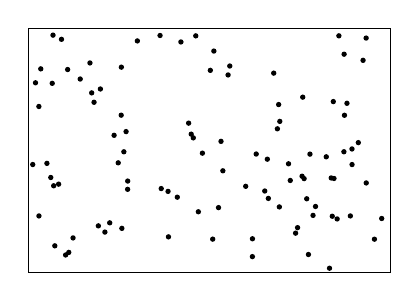
\begin{tikzpicture}[scale=1.5]
        \draw (-1pt,-1pt) rectangle ($(3,2)+(1pt,1pt)$);
        \pgfmathsetseed{1}
        \foreach \i in {1,2,...,100}{
            \draw[fill=black] (rnd*3,rnd*2) circle[radius=.5pt];
        };
    \end{tikzpicture}
}

% Two chambers separated by a piston
\newcommand{\tfigTwoChambersSeparatedByPiston}{
    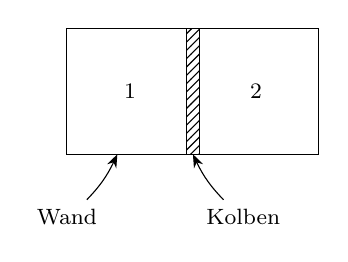
\begin{tikzpicture}[scale=1.6]
        \draw (0,0) rectangle (2,1);
        \node at (.5,.5) {1};
        \node at (1.5,.5) {2};
        \draw[pattern=north east lines] (.95,0) rectangle (1.05,1);
        \node at (0,-.5) {Wand} edge[arr,bend right=10] (.4,0);
        \node at (1.4,-.5) {Kolben} edge[arr,bend left=10] (1,0);
    \end{tikzpicture}
}

% Rectangular box with piston
\newcommand{\tfigRectangularBoxWithPiston}{
    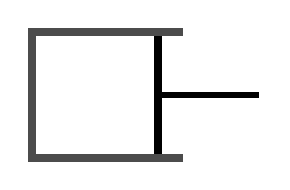
\begin{tikzpicture}[scale=1.6]
        \draw[line width=3pt] (1,0) -- (1,1);
        \draw[line width=2pt] (1,.5) -- +(.8,0);
        \draw[draw=black!70!white,line width=3pt] (1.2,0) -- (0,0) -- (0,1) -- (1.2,1);
    \end{tikzpicture}
}

% Water with ice cubes. Stiring heats up the water and ice cubes vanish
\newcommand{\tfigWaterStiringIceCubes}{
    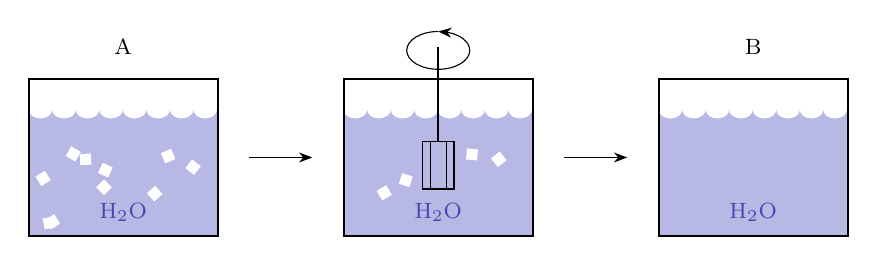
\begin{tikzpicture}[water color/.style={nice light blue},wave deco/.style={decoration={bumps,amplitude=-3,segment length=17}},scale=2]
        \begin{scope}
            \fill[blue!20!white!90!black] decorate[wave deco] {(0,.8) -- (1.2,.8)} -- (1.2,0) -- (0,0) -- (0,.8);
            \draw[thick] (0,0) rectangle (1.2,1); 
            \pgfmathsetseed{5}
            \foreach \i in {1,2,...,10} {
                \coordinate (A) at (rnd+.1,rnd*.5+.1);
                \fill[color=white,rotate around={rnd*360:(A)}] (A) rectangle +(2pt,2pt);
            };
            \node[water color] at (.6,.15) {$\mathrm{H}_2\mathrm{O}$};
            \node at (.6,1.2) {A};
        \end{scope}
        \draw[arr] (1.4,.5) -- +(.4,0); 
        \begin{scope}[xshift=2cm]
            \fill[blue!20!white!90!black] decorate[wave deco] {(0,.8) -- (1.2,.8)} -- (1.2,0) -- (0,0) -- (0,.8);
            \draw[thick] (0,0) rectangle (1.2,1); 
            \foreach \i in {1,2,...,4} {
                \coordinate (A) at (rnd+.1,rnd*.5+.1);
                \fill[color=white,rotate around={rnd*360:(A)}] (A) rectangle +(2pt,2pt);
            };
            \node[water color] at (.6,.15) {$\mathrm{H}_2\mathrm{O}$};
            
            \draw (.5,.3) rectangle +(.2,.3) (.55,.3) rectangle +(.1,.3);
            \draw[thick] (.6,.6)-- +(0,.6);
            \draw[arr] (.6,1.3) arc[x radius=.2, y radius=.12,start angle=-270, end angle=90];
        \end{scope}
        \draw[arr] (3.4,.5) -- +(.4,0); 
        \begin{scope}[xshift=4cm]
            \fill[blue!20!white!90!black] decorate[wave deco] {(0,.8) -- (1.2,.8)} -- (1.2,0) -- (0,0) -- (0,.8);
            \draw[thick] (0,0) rectangle (1.2,1);
            \node[water color] at (.6,.15) {$\mathrm{H}_2\mathrm{O}$};
            \node at (.6,1.2) {B};
        \end{scope}
    \end{tikzpicture}
}

% Visualize that W,Q are no state functions. Adding different ratios of W and Q to a system may lead to the same inner energy U. 
\newcommand{\tfigWQAreNoStateFunctions}{
    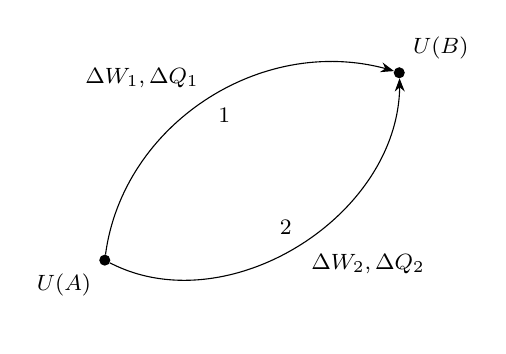
\begin{tikzpicture}[scale=1.7]
        \node[point,label={north east}:$U(B)$] (Point B) at (2.2,1.4) {};
        \node[point,label={south west}:$U(A)$] (Point A) at (0,0) {} 
        edge[arr,bend left=50] node[midway, anchor=south east] {$\Delta W_1,\Delta Q_1$} node[midway, anchor=north west] {1} (Point B)
        edge[arr,bend right=60] node[midway, anchor=north west] {$\Delta W_2,\Delta Q_2$} node[midway, anchor=south east] {2} (Point B);
    \end{tikzpicture}
}